%!TEX encoding = IsoLatin

\documentclass[12pt]{ULrapport}
\usepackage[ansinew]{inputenc}
\usepackage[french]{babel}
\usepackage{float}
\restylefloat{table}
\usepackage{hhline}
\usepackage{pdfpages}
\usepackage{hyperref}


% Title Page
\title{Design III: Pirates des Cara�bes}
\author{ Charles-Olivier Magnan, Jean-Michel Provencher}



\TitreProjet{Design III}                       
\TitreRapport{Remise 1}                      
\Destinataire{ Philippe Gigu�re, Dominique Grenier, Denis Laurendeau}         
\NumeroEquipe{7}                                     
\NomEquipe{Zi�re}                               
\TableauMembres{%
	111\,114\,478  & Garvin, S�bastien   & \\\hline 
	111\,040\,128  & Kedzierski, Xavier   & \\\hline     
	111\,066\,466  & Magnan, Charles-Olivier      & \\\hline
	111\,071\,384  & Provencher, Jean-Michel   & \\\hline     
	111\,073\,630	 & Bourque, Emile						& \\\hline
	111\,075\,478	 & Sylvain, Matthieu			& \\\hline
	111\,074\,361  & Brown, J�r�my				& \\\hline
	907\,196\,009  & Garneau, Laurent			& \\\hline
}
\DateRemise{31 janvier 2016} 
% Contenu de l'historique des versions
\HistoriqueVersions{%										% version & date & description \\\hline
       1.0  & 24 janvier 2016 & Cr�ation du document \\\hline
			 2.0  & 31 janvier 2016 & Remise 1 \\\hline
			}

\begin{document}

% Chapitres
\chapter{Diagrammes}
\label{s:Diagrammes}


\section{Diagramme de contexte}
\label{s:Diagramme_contexte}

\begin{figure}[htp]
   \centering
   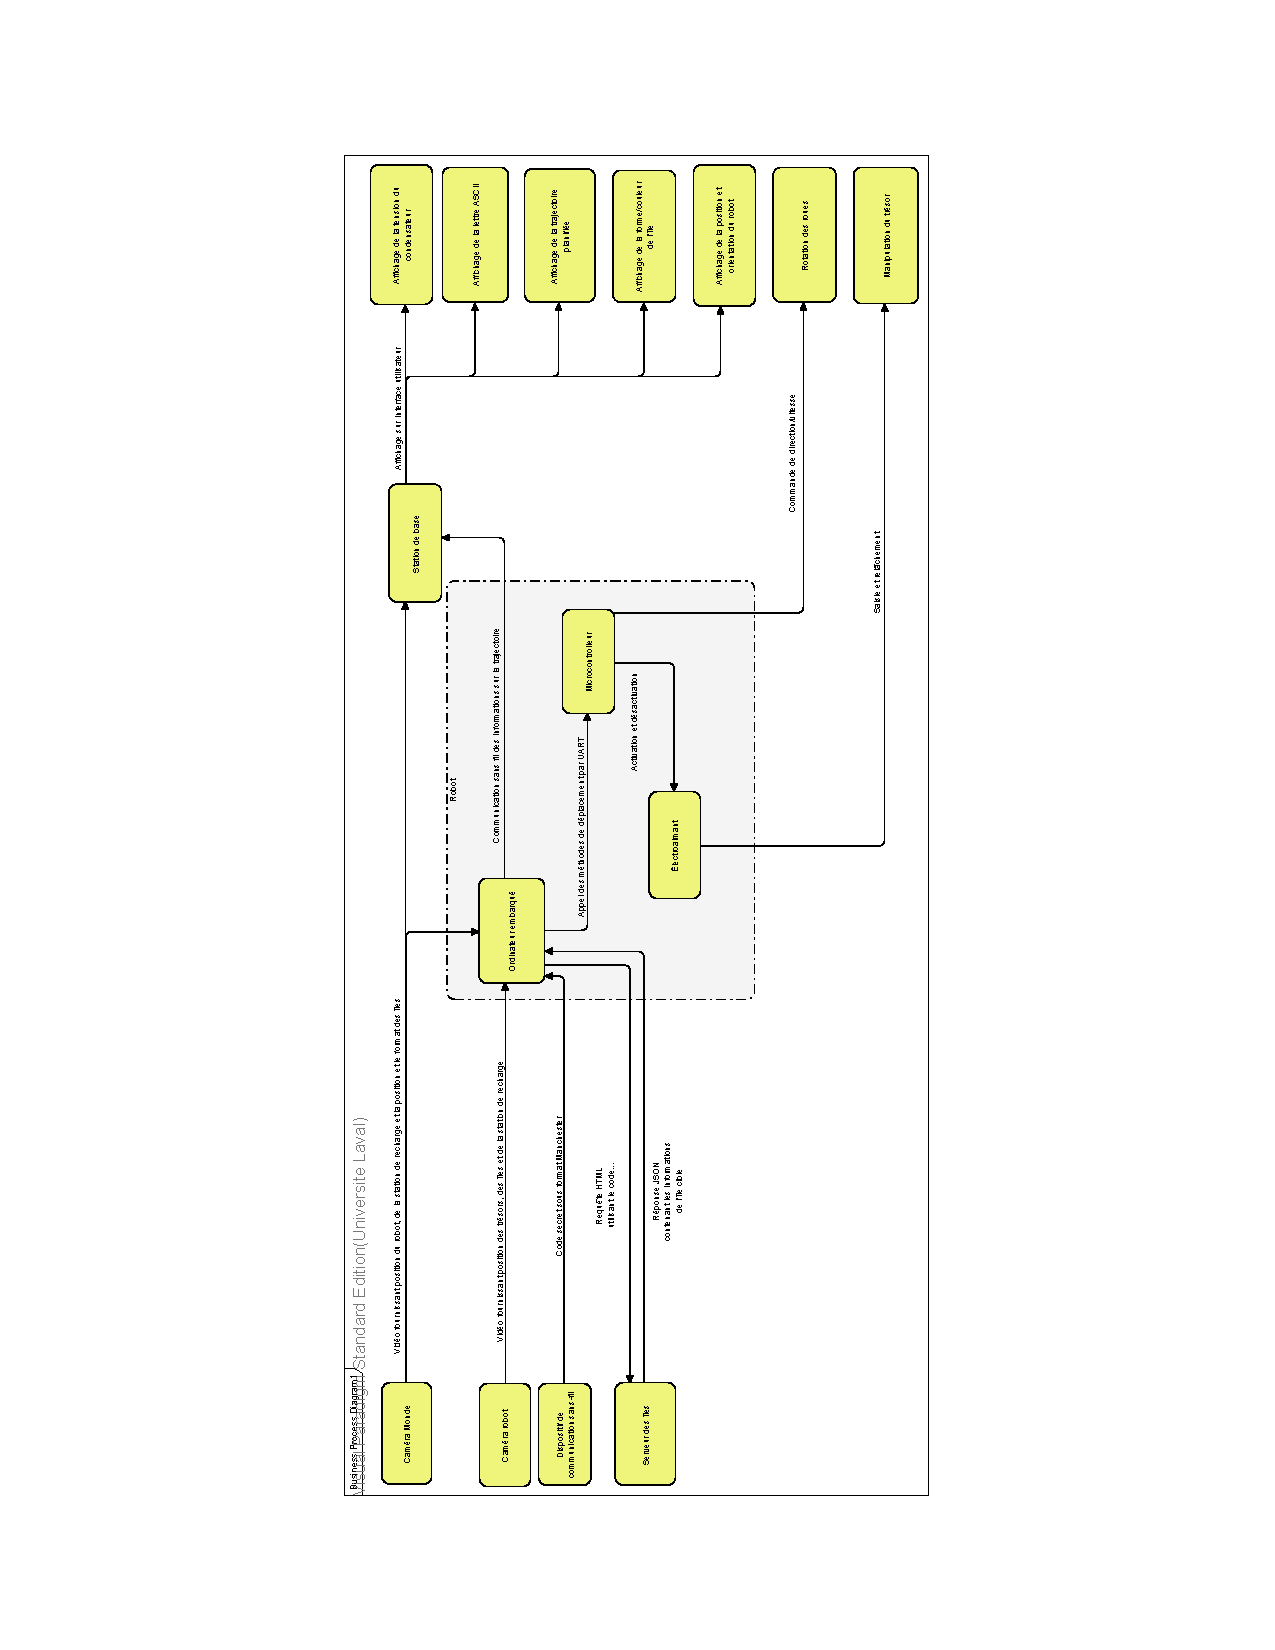
\includegraphics[width=0.75\textwidth, angle =-90]{pdf/ContextDiagram.pdf}
   \caption{Diagramme de contexte}
   \label{f:Diagramme_contexte}
\end{figure}

\newpage

\section{Diagramme de classes}
\label{s:Diagramme_classes}

\begin{figure}[htp]
   \centering
   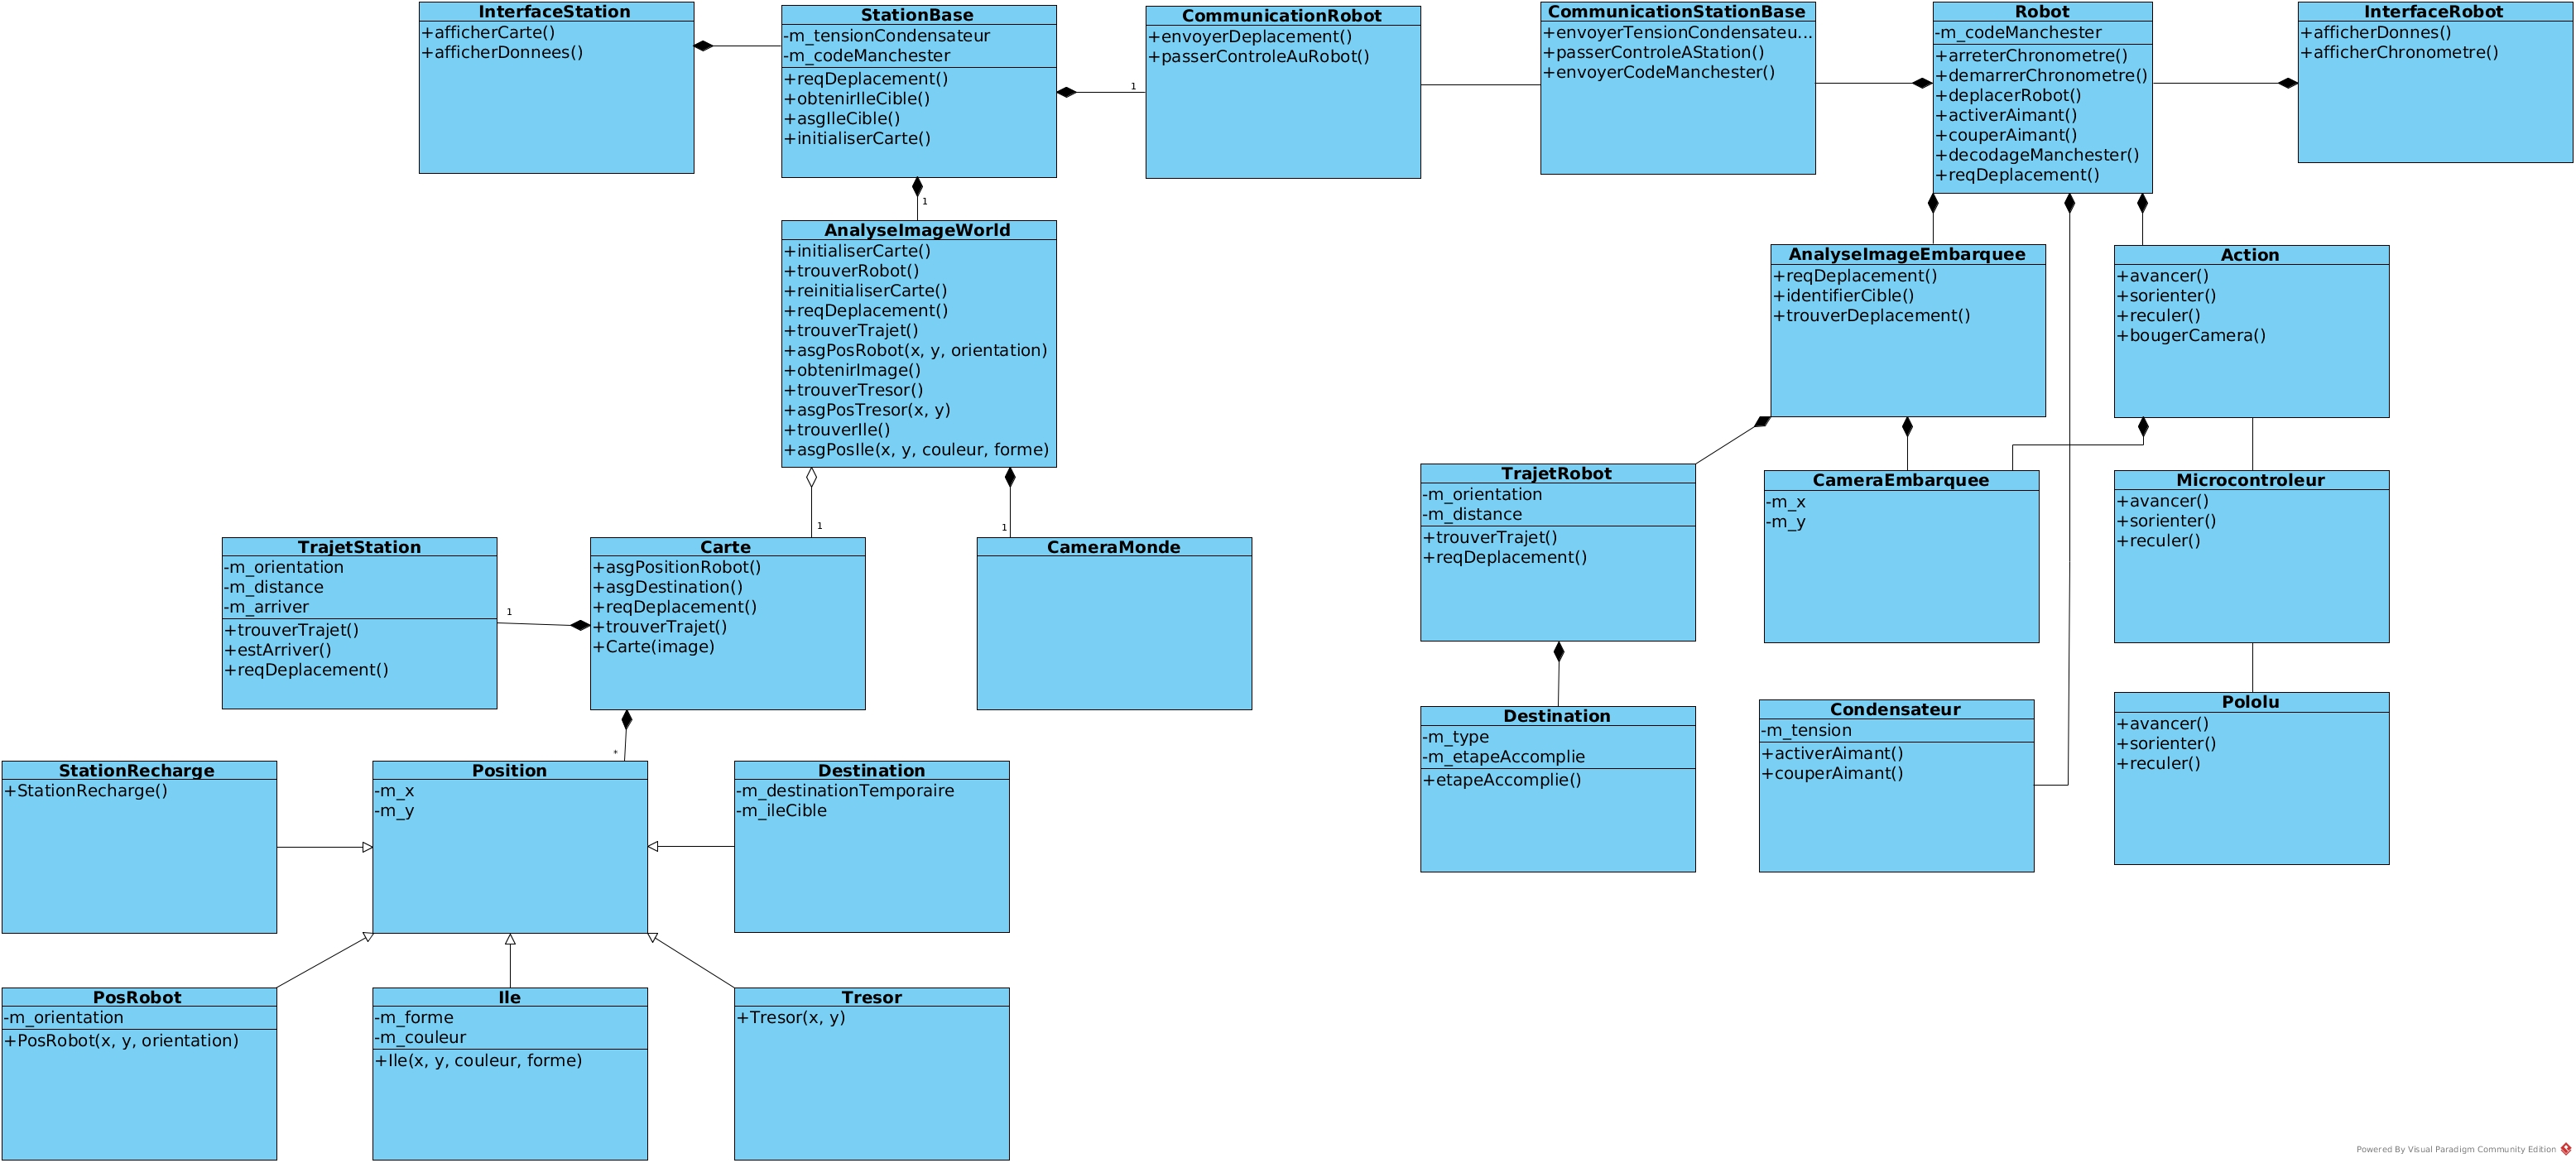
\includegraphics[width=0.95\textwidth, angle =-90]{fig/ClassDiagram.jpg}
   \caption{Diagramme de classes}
   \label{f:Diagramme_Classes}
\end{figure}

\newpage


La figure \ref{f:Diagramme_Classes} repr�sente le diagramme de classes suite � la premi�re it�ration. La structure est suseptible de changer suite aux prochaine it�rations, mais voici une br�ve description de la structure sur laquelle nous nous entendons pr�sentement. \par

La section de gauche du diagramme sera impl�ment�e sur la station de base tandis que la section droite sera impl�ment�e sur le robot. Ces deux syst�me pouront communiquer entre eux � l'aide des classes CommunicationRobot et CommunicationStationBase. \par

En ce qui conscerne la station de base, le contr�leur du syst�me est repr�sent� par la classe StationBase. La classe AnalyseImageWorld analyse les images re�u de la CameraMonde et g�n�re une carte sh�matique de la table (Carte) � l'aide d'imagerie. La carte est compos�e de diverses �l�ments qui h�rite tous de la classe Position. Les trajectoires du robot seront calcul� dans la classe TrajetStation � l'aide des informations de la classe Carte.  \par

Pour ce qui est du robot, il est aussi compos� d'un contr�leur (Robot). Les mouvements que devra effectuer le robot passerons tous par la classe Action qui les acheminera au microcontroleur et au polulu si nescessaire. Lorsque le robot est pr�s de la destination, TrajetRobot calculera les trajets (� l'aide de Destination et d'imagerie effectu� dans AnalyseImageEmbarquer).

    
   



\section{Diagramme de s�quences}
\label{s:Diagramme_sequences}

\begin{figure}[htp]
	\centering
	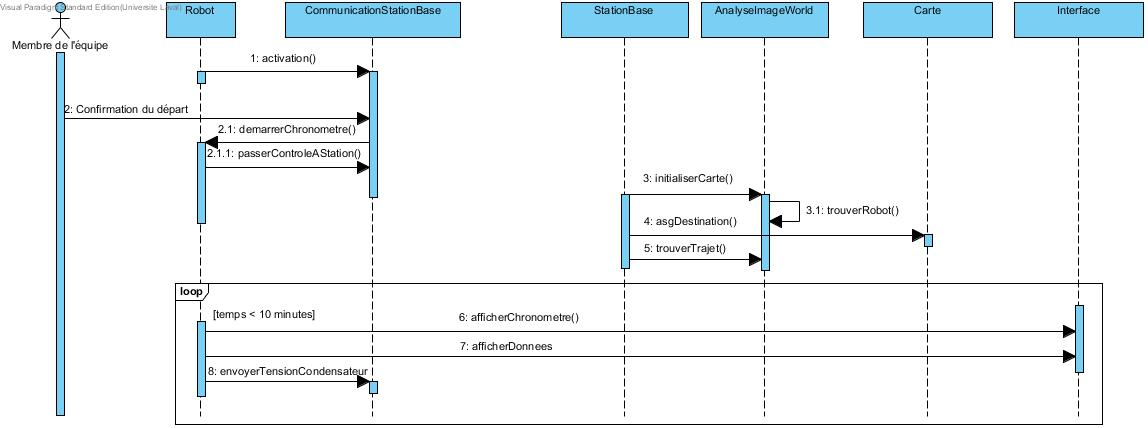
\includegraphics[width=0.95\textwidth]{fig/demarrageRobot.jpg}
	\caption{D�marrage du Robot}
	\label{f:DemRob}
\end{figure}

%\begin{figure}[htp]
%   \centering
%   \includegraphics[width=1\textwidth]{Diagramme_sequences}
%   \caption{Diagramme de s�quences}
%   \label{f:Diagramme_sequences}
%\end{figure}


\chapter{Description des cas d'utilisation}
\label{s:Description_Utilisation}



\section{Diagramme des cas d'utilisation}

\begin{figure}[htp]
\centering
	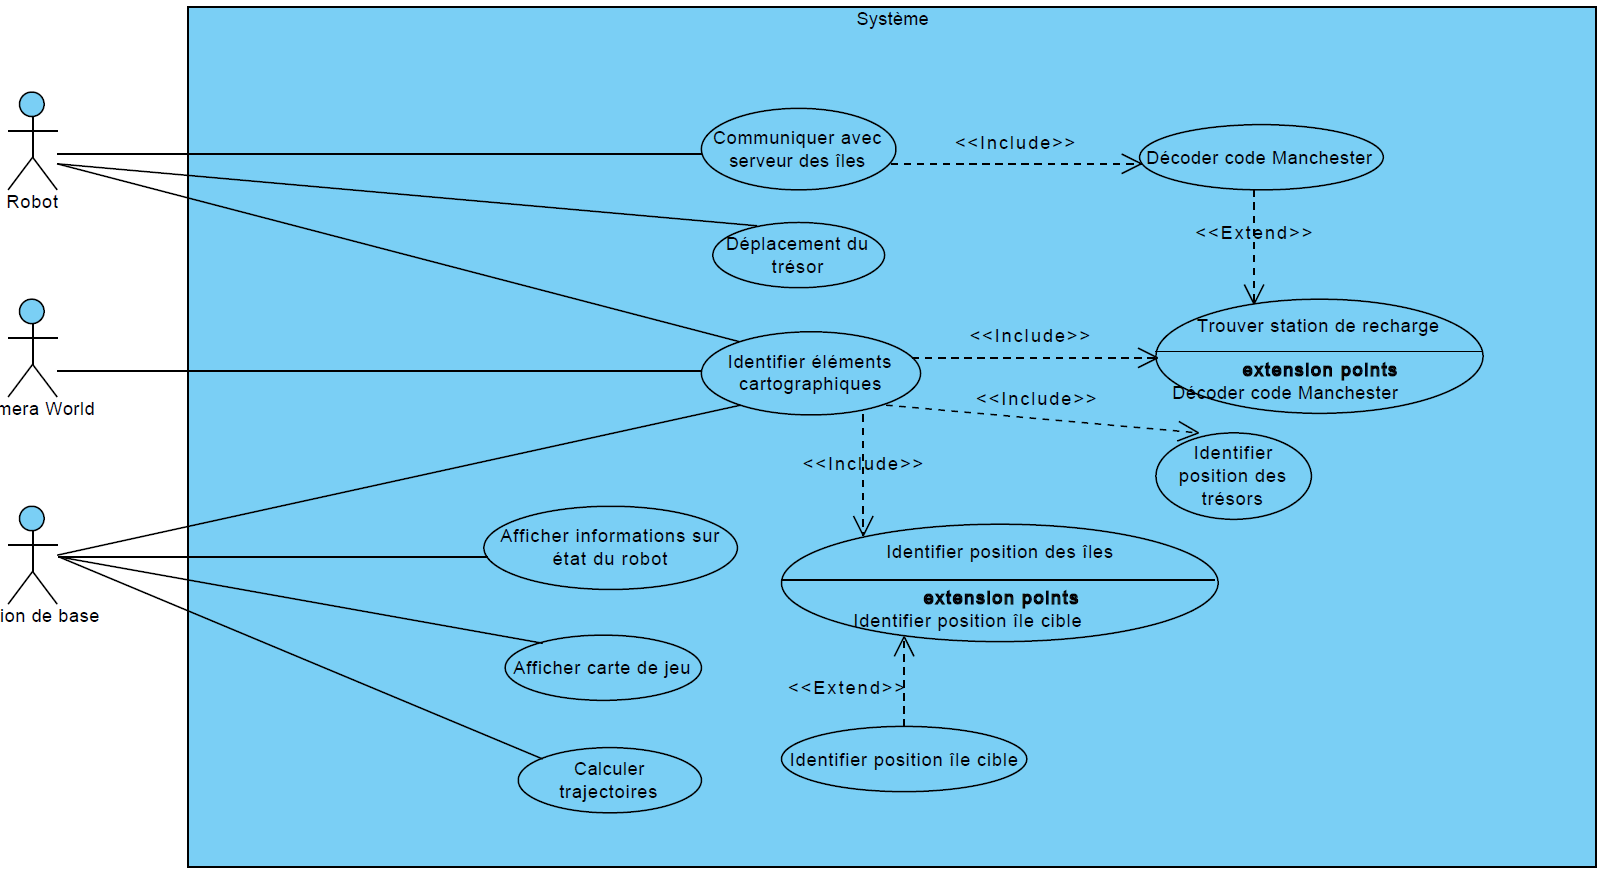
\includegraphics[width = 0.8\textwidth]{fig/casutilisation.png}
	\label{fig:Cas_Utilisation}
	\caption{Diagramme des cas d'utilisation}
\end{figure}


\pagebreak


\section{Sc�narios des cas d'utilisation}
%%%%%%%%%%%%%%% CAS UTILISATION 1 %%%%%%%%%%%%%%%%%
	%%%%%%%%%%% Identifier les �l�ments cartographiques  %%%%%%%%%%%%%
	%%%%%%%%%%%%% ETAT: A COMPLETER %%%%%%%%%%%%%%%%%%%%%%
    \begin{table}[!ht]
    \caption{Cas d'utilisation - Identifier les �l�ments cartographiques}
    \begin{tabular}{| l | p{4.75cm} p{4.75cm} |}
    \hline
    Cas d'utilisation & \multicolumn{2}{p{9.5cm} |}{Identifier les �l�ments cartographiques} \\ \hline
    Syst�me & \multicolumn{2}{p{9.5cm} |}{Syst�me de reconnaissance visuelle}\\ \hline
    Acteurs & \multicolumn{2}{p{9.5cm} |}{Robot, cam�ra world, station de base}\\ \hline
    Partie prenante et int�r�t & \multicolumn{2}{p{9.5cm} |}{Station de base : Vouloir identifier les �l�ments pr�sents sur la carte afin que le robot puisse remplir son mandat.}\\ 
    \hline
    Pr�conditions & \multicolumn{2}{p{9.5cm} |}{Le robot et la cam�ra world doivent fournir des images � la station de base}\\ \hline
    Garantie en cas de succ�s & \multicolumn{2}{p{9.5cm} |}{Les �l�ments cartographiques sont affich�s sur la carte de la station de base}\\ \hline
    
    \multirow{4}{*}{Sc�nario principal} 
    
    & 1. Big show baby & \\
    & & 2. Big show 2 baby \\
    & & 3.  Showtime \\
    & 4. Uiuuu & \\
    
    \hline
    
    \multirow{1}{*}{Sc�narios alternatifs} 
    
    & Aucun sc�nario alternatif & \\
    
    \hline
    \end{tabular}
    \label{tab:identifier_elements_cartes}
    \end{table}
    
    
%%%%%%%%%%%%%%% CAS UTILISATION 2 %%%%%%%%%%%%%%%%%
	%%%%%%%%%%% Trouver station de recharge  %%%%%%%%%%%%%
	%%%%%%%%%%%%% ETAT: A COMPLETER %%%%%%%%%%%%%%%%%%%%%%
    \begin{table}[!ht]
    \caption{Cas d'utilisation - Trouver la station de recharge}
    \begin{tabular}{| l | p{4.75cm} p{4.75cm} |}
    \hline
    Cas d'utilisation & \multicolumn{2}{p{9.5cm} |}{Trouver station de recharge} \\ \hline
    Syst�me & \multicolumn{2}{p{9.5cm} |}{Syst�me de reconnaissance visuelle}\\ \hline
    Acteurs & \multicolumn{2}{p{9.5cm} |}{Robot, cam�ra world, station de base}\\ \hline
    Partie prenante et int�r�t & \multicolumn{2}{p{9.5cm} |}{Robot : Faire le plein d'�nergie et recevoir le code Manchester}\\ 
    \hline
    Pr�conditions & \multicolumn{2}{p{9.5cm} |}{La station de base a identifi� la position de la station de recharge et une trajectoire a �t� calcul�e}\\ \hline
    Garantie en cas de succ�s & \multicolumn{2}{p{9.5cm} |}{La trajectoire menant le robot jusqu'� la station de recharge est affich�e sur la station de base. Le robot se d�place vers la station de recharge sans toucher � aucun obstacle.}\\ \hline
    
    \multirow{4}{*}{Sc�nario principal} 
    
    & 1. Big show baby & \\
    & & 2. Big show 2 baby \\
    & & 3.  Showtime \\
    & 4. Uiuuu & \\
    
    \hline
    
    \multirow{1}{*}{Sc�narios alternatifs} 
    
    & Aucun sc�nario alternatif & \\
    
    \hline
    \end{tabular}
    \label{tab:trouver_station_recharge}
    \end{table}



\chapter{Familiarisation avec �quipements et exp�riences pr�liminaires}
\label{s:Familiarisation_Experiences}


\section{Structure m�canique}
\label{s:Structure_mecanique}



\section{Syst�me de pr�henseur et d'�lectroaimant}
\label{s:Prehenseur}



\section{Station de recharge}
\label{s:Station_recharge}



\section{Asservissement des moteurs}
\label{s:Controle_moteurs}

Afin de commander les moteurs du robot, il est n�cessaire d'avoir une routine d'asservissement. Afin de communiquer les commandes avec les moteurs DC, l'Arduino Mega est choisi. Celui-ci poss�de une vitesse d'horloge de 16 MHz et 256kB de m�moire flash pour 45\$ \cite{MEG00}, ce qui est un bon �quilibre performance/prix pour les besoins du projet.
\medbreak
Les moteurs utilis�s pour entra�ner les roues du robot poss�dent 6400 valeurs de position par rotation. Si une interruption est effectu�e � chaque modification de cette valeur, on risque d'emp�cher l'ex�cution compl�te d'une boucle d'asservissement entre deux interruptions. Donc, si une interruption est lev�e � chaque modification de la position, il faut s'assurer que le calcul de la vitesse de rotation se fasse apr�s un nombre multiple d'interruptions, avec un compteur de temps.
\medbreak
Pour ce qui a trait � la communication avec les moteurs DC, un shield Adafruit se connectant directement sur l'Arduino Mega est utilis�. Avec celui-ci, il est possible de g�n�rer des ondes modul�es (PWM) servant � contr�ler les quatres roues individuellement, avec chacun une r�solution de 8 bits et jusqu'� 1.2 amp�res par canal\cite{SLD00}. Cette division de la commande est utile lors d'un d�placement en diagonale, et pourrait �galement �tre utile pour continuer le fonctionnement dans le cas d'une roue d�fectueuse. Ce dispositif est utilis� pour contr�ler les moteurs pour les premiers tests, bien �videmment l'utilisation du pont en H fournit fera aussi l'objet de tests.
\medbreak
En r�sum�, l'ordinateur envoie des instructions de direction au microcontr�leur Arduino, qui ex�cute alors une routine de d�placement. Celle-ci est bas�e sur un asservissement de vitesse, d�termin�e par des interruptions lors de la rotation des servomoteurs. Les commandes de l'Arduino sont alors communiqu�es aux roues � l'aide d'un shield Adafruit permettant de leur d�livrer de la puissance.



\section{Localisation du robot et des �les}
\label{s:Localisation_Robot_Iles}



\section{Rep�rage des tr�sors et de la station de recharge}
\label{s:Reperage}

La cam�ra Logitech C905 situ�e sur le robot permettra de rep�rer les diff�rents tr�sors ainsi que la station de recharge. Cette cam�ra sera contr�l�e par les Servomoteurs fournis qui permettront � la cam�ra un d�placement sur son axe horizontal et vertical afin d'augmenter le champ de vision du robot. Afin de contr�ler le � Polulu � Maestro 6-Channel USB Servo Controller, des commandes seront envoy�es par USB � partir de l'ordinateur embarqu� situ� sur le robot. La cam�ra embarqu�e sera �galement reli�e directement � l'ordinateur embarqu�e afin d'�tre aliment�e et de fournir les images capt�es. La fr�quence de captation des images reste � d�terminer puisqu'il faudra d�cider � quel intervalle nous devons mettre � jour la vision du robot. L'envoi des commandes afin de contr�ler la prise d'image par la cam�ra sera effectu�e par la librairie Pygame en Python.

Afin de d�tecter les tr�sors, une premi�re approximation de leur position est effectu�e par la cam�ra monde qui, � l'aide de la librairie cv2 de OpenCV, permet de localiser dans une image un intervalle de couleur BGR. Le choix de la librairie d'OpenCV est justifi� par le fait qu'elle poss�de toutes les fonctions n�cessaires � un programme de vision complet et qu'elle s'int�gre facilement au reste du code en Python. Les tests effectu�es avec la cam�ra monde ont permis de venir � la conclusion que la d�tection des tr�sors s'effectuent tr�s bien. Par contre, les tests ont �galement permis de constater que la cam�ra monde ne voit pas le fond de la table et donc, certains tr�sors ne seront pas d�tecter par la cam�ra monde, justifiant la d�tection des tr�sors �galement par la cam�ra embarqu�e. Par la suite, les diff�rents pixels correspondant � la couleur des tr�sors sont plac�s dans un masque des tr�sors. Gr�ce � la position relative de ces points dans le masque des tr�sors, il est possible d'avoir une position approximative de ces tr�sors dans la carte virtuelle. Afin de confirmer la d�tection de ces tr�sors ou pour rep�rer les tr�sors qui seront hors du champ de vision du robot, la m�me op�ration de d�tection des couleurs est effectu�e ensuite par la cam�ra embarqu�e autour des coordonn�es approximative d�tect�e par la cam�ra monde.

La station de recharge, quant � elle, est marqu�e d'une couleur caract�ristique lui permettant de se distinguer du reste du d�cor. Comme la position et l'orientation du robot est connue en tout temps et que la station de recharge est toujours situ� au m�me endroit, la d�tection de celle-ci est assez simple. Comme le robot peut �tre plac� � n'importe quel endroit au d�part sur la table, la cam�ra monde est charg�e � l'initialisation du programme de d�tecter la position et l'orientation de celui-ci. Afin de r�aliser cette t�che, un drapeau pirate est plac� sur le dessus du robot afin d'indiquer l'orientation ainsi que la position de celui-ci et sera d�tecter par notre programme de vision.




\section{Alimentation du robot}
\label{s:Alimentation}



\section{Communications sans fil}
\label{s:Communication}



%Autres sections au choix selon ce qui sera d�cid�
%%!TEX encoding = IsoLatin

%
% Chapitre "Introduction"
%

%Sites d'achats, factures, etc


\begin{thebibliographyUL}{99} % remplacer le "{9}" par "{99}" lorsque le nombre de references
                              % requiert 2 caracteres (>= 10 references)
\bibitem{MOD00} Design II (mod�lisation), \textit{Actionneur �lectromagn�tique Partie 2}, [En ligne], \url{http://wcours.gel.ulaval.ca/2015/h/GEL2007/default/5notes/Seminaire_Actionneur_Balance_2015_part2fin.pdf}, Page consult�e le 17 f�vrier 2015

\end{thebibliographyUL}

%\appendix
%%!TEX encoding = IsoLatin

%
% Annexe "Liste des sigles et des acronymes"
%

\chapter{Liste des sigles et des acronymes}
\label{Sigles}

\begin{flushleft}
   \begin{tabular}{@{}ll}
      \textbf{CAO}        & Conception Assist�e par Ordinateur \\
   \end{tabular}
\end{flushleft}



\end{document}          
